\chapter{Introduction}\label{chap:intro}
The Exascale Grid Optimization (ExaGO\texttrademark) toolkit is an open source package for solving large-scale power grid optimization problems on parallel and distributed architectures, particularly targeted for exascale machines with heteregenous architectures (GPU). ExaGO\texttrademark~is written in C/C++ and makes heavy use of the functionality provided by the PETSc\cite{petsc-user-ref} library. It uses \raja and \umpire libraries for execution on the GPU and can make use of several optimization solvers - \ipopt, \hiop - for solving the optimization problems.


All ExaGO\texttrademark~applications use a nonlinear formulation based on full AC optimal power flow. The different applications available with \exago are listed in Table \ref{tab:exago_apps}

\begin{table}[!htbp]
    \centering
  \caption{\exago applications}
  \begin{tabular}{|l|p{0.4\textwidth}|p{0.3\textwidth}|}
    \hline
    \textbf{Application} & \textbf{Description} & \textbf{Notes} \\
    \hline
    \opflow & AC optimal power flow & \\ \hline
    \scopflow & Security-constrained AC optimal power flow & Uses \tcopflow for multi-period contingencies \\ \hline
    \tcopflow & Multi-period AC optimal power flow & \\ \hline
    \sopflow & Stochastic AC optimal power flow & Uses \scopflow for multi-contingency scenarios \\
    \hline
%    \pflow & AC power flow & \\ \hline
  \end{tabular}
  \label{tab:exago_apps}
\end{table}

While \exago is targeted for making use of distributed computing environments and GPUs, its full support is still under development. Table \ref{tab:exago_apps_arch} lists the architecure support for ExaGO applications.

%\tcopflow can only run on a single CPU process. \scopflow and \sopflow can run in parallel on multiple CPU processes, but they can only execute independent ACOPFs for contingencies and scenarios. Solving the full SCOPF and Stochastic OPF problem in a parallel setting is under development. \opflow execution on the GPU has only been tested with NVIDIA GPUs. 

\begin{center}
\begin{table}[!htbp]
    \centering
    \caption{\exago application execution on different hardware}
    \begin{tabular}{|c|c|c|c|}
      \hline
      \textbf{Application} & \textbf{CPU (serial)} & \textbf{CPU (parallel)} & \textbf{GPU} \\
      \hline
      \opflow   & Y & N & Y \\ \hline
      \scopflow & Y & Y  & Y \\ \hline
      \sopflow  & Y & Y  & Y \\ \hline
      \tcopflow & Y & N & N \\ \hline
%      \pflow    & Y & Y & N \\ \hline
    \end{tabular}
    \label{tab:exago_apps_arch}
\end{table}
\end{center}

\noindent
Together, these applications cater to problems spanning the dimensions of security (contingencies), stochasticity, and time as shown in Figure \ref{fig:intro_fig}.

\tikzstyle{vtx}=[draw,circle,fill,minimum width=1pt]

\tikzstyle{ed}=[color=blue]

\begin{figure}[h!]
    \centering
    \scalebox{.8}{

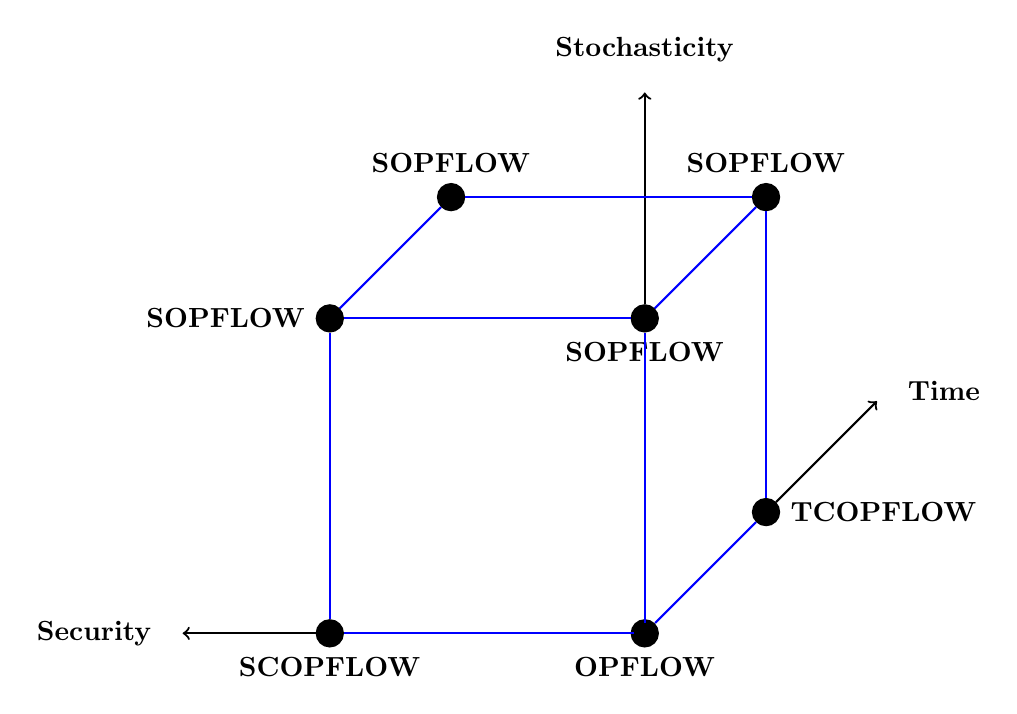
\begin{tikzpicture}[auto, thick]
   \node (o) at (0,0,0) {};
   \node[label=left:{\textbf{Security}}] (x) at (-6,0,0) {}; 
   \node[label=above:{\textbf{Stochasticity}}] (y) at (0,7,0) {}; 
   \node[label=right:{\textbf{Time}}] (z) at (0,0,-8) {}; 
 % \node[time,label=below:$t_0$] (t0) at (0,0) {};
 % \node[time,label=below:$t_1$] (t1) at (2,0) {};
 % \node[time,label=below:$t_2$] (t2) at (4,0) {};
 % \node[time,label=below:$t_3$] (t3) at (6,0) {};
  
  \node[vtx,label=below:\textbf{OPFLOW}] (opflow) at (0,0,0) {};
  \node[vtx,label=right:\textbf{TCOPFLOW}] (tcopflow) at (0,0,-4) {};
  \node[vtx,label=below:\textbf{SCOPFLOW}] (scopflow) at (-4,0,0) {};
  \node[vtx,label=below:\textbf{SOPFLOW}] (sopflow) at (0,4,0) {};
  

  \node[vtx,label=above:\textbf{SOPFLOW}] (b) at (0,4,-4) {};
  \node[vtx,label=left:\textbf{SOPFLOW}] (c) at (-4,4,0) {};
  \node[vtx,label=above:\textbf{SOPFLOW}] (d) at (-4,4,-4) {};
  
  \path (scopflow) edge [->,thick] (x);
  \path (sopflow) edge [->,thick] (y);
  \path (tcopflow) edge [->,thick] (z);
  
  \path (sopflow) edge [ed] (b);
  \path (sopflow) edge [ed] (c);
  \path (b) edge [ed] (d);
  \path (c) edge [ed] (d);
  
  \path (scopflow) edge [ed] (c);
  \path (tcopflow) edge [ed] (b);
  \path (o) edge [ed] (tcopflow);
  \path (o) edge [ed] (scopflow);
  \path (o) edge [ed] (sopflow);
 % \path (t0) edge (t1);
 % \path (t1) edge (t2);
 % \path (t2) edge (t3);


\end{tikzpicture}}
\caption{\exago provides applications along the dimensions of security (contingencies), time, and stochasticity. The label vertices denote different \exago applications available.}
\label{fig:intro_fig}
    
\end{figure}



